\section*{Analysis of Merge-Sort}

The correctness of the algorithm can be proved by induction, as the natural structure of above algorithm is recursive.
Specifically, we want to prove the statement that the merge-sort function with $A$ as input returns the sorted array of $A$ if $|A| = n$.
The induction is w.r.t.\ $n$. The base case, i.e., $n = 1$, is clearly correct.
In the inductive step, we assume that above statement is true for $|A| = 1, 2, \cdots, n - 1$, and we aim to prove it is correct for $|A| = n$.
As the algorithm is correct for $|A| = 1, 2, \cdots, n - 1$, in particular, it is correct for $|A| = n/2$, i.e.,
$S'_1$ and $S_2'$ store the sorted array of $S_1$ and $S_2$, respectively.
Combinining the correctness of merge-two-sorted-arrays that we have already proved,
we have that merge-sort returns the sorted array of $S$.

To see its runing time, we define $T(n)$ as the running time of merge-sort~($S$) when $|S| = n$.
Clearly, both merge-sort~($S[1\cdots n/2]$) and
merge-sort~($S[n/2+1\cdots n]$) take $T(n/2)$ time.
As merge-two-sorted-arrays takes linear time, we have the recurrence $T(n) = 2T(n/2) + \Theta(n)$.
We will use \emph{master's theorem} to get the closed form for $T(n)$, described below.

\section*{Master's Theorem}

Master's theorem gives closed form for the following recurrence:
\begin{displaymath}
T(n) = \left\{
\begin{array}{llll}
aT(n/b) + \Theta(n^d)  & \textrm{ if } n \ge 2 \\
1  & \textrm{ if } n \le 1 
\end{array}
\right.
\end{displaymath}

Master's theorem is widely used to analyze the running time of divide-and-conquer algorithms. 
Recall that a divide-and-conquer algorithm
first partitions the original problems into subproblems, solve all subproblems recursively,
and then combine them to answer the original question.
Hence, above recurrence precisely describes the running time of such algorithms.
Specifically, $a$ refers to the number of subproblems that the original problem is partitioned,
$n/b$ refer to the input-size of each subproblem,
and $\Theta(n^d)$ refer to the running time of the combining step.
In merge-sort, $a = 2$, as it calls merge-sort twice in the algorithm,
$b = 2$, as the input-size of each subproblem becomes $n/2$,
and $d = 1$, as the merge-two-sorted-arrays takes $\Theta(n)$ time.
Note that, it is not always the case that $a = b$~(in merge-sort though, $a = b$).
Such example includes matrix multiplication.

We now solve above recurrence. Without loss of generality, we assume that $n$ is a power of $b$, i.e., $n = b^k$ for some $k$.
To further simplify, we use $n^d$ instead of $\Theta(n^d)$.
We therefore need to add $\Theta(\cdot)$ to the resulting formular of $T(n)$.

\begin{eqnarray*}
T(n) & = & aT(n/b) + n^d \\
     & = & a(aT(n/b^2) + (n/b)^d) + n^d \\
	 & = & a^2 T(n/b^2) + a(n/b)^d + n^d \\
     & = & a^2(aT(n/b^3) + (n/b^2)^d) + a(n/b)^d + n^d \\
	 & = & a^3 T(n/b^3) + a^2(n/b^2)^d + a(n/b)^d + n^d \\
	 & = & \cdots \\
	 & = & a^k T(n/b^k) + \sum_{i = 0}^{k-1} a^i(n/b^i)^d
\end{eqnarray*}

As we assume that $n = b^k$ and $T(1) = 1$, we have
$$ T(n) =  a^k + \sum_{i = 0}^{k-1} a^i(n/b^i)^d = \sum_{i = 0}^{k} a^i(n/b^i)^d = n^d \sum_{i = 0}^{k} (a/b^d)^i.$$

Consider the following 3 cases. 
\vspace*{-\topsep}
\begin{enumerate}
\item If $a = b^d$, i.e., $d = \log_b a$, then $T(n) = n^d k = n^d \log_b n = \Theta(n\log n)$.
\item If $a < b^d$, i.e., $d > \log_b a$, then the series decreases exponentially, and therefore the item of $i = 0$ dominates.  $T(n) = n^d a/b^d = \Theta(n^d)$.
\item If $a > b^d$, i.e., $d < \log_b a$, then the series increases exponentially, and therefore the item of $i = k$ dominates.  
$T(n) = n^d (a/b^d)^k = n^d a^k / b^{dk} = n^d a^k/n^d = a^k = a^{\log_b n} = n^{\log_b a}$.
\end{enumerate}

We have used one facts about logarithmic function above: %$\log_b n = \log_b 2 \cdot \log_2 n$, and 
$a^{\log_b n} = n^{\log_b a}$.

Master's theorem can be summarized as below. For recurrence $T(n) = aT(n/b) + n^d$ with $T(1) = 1$, we have the following:
\begin{displaymath}
T(n) = \left\{
\begin{array}{llll}
\Theta(n^d \log n) & \textrm{ if } d = \log_b a \\
\Theta(n^d) & \textrm{ if } d > \log_b a \\
\Theta(n^{\log_b a}) & \textrm{ if } d < \log_b a \\
\end{array}
\right.
\end{displaymath}

In the case of merge-sort, $a = b = 2$ and $d = 1$. So $d = \log_b a = 1$.
Hence, $T(n) = \Theta(n\log n)$.

A more generalized form of master's theorem is to solve this recurrence:
$T(n) = aT(n/b) + n^d \log^s n$ with $T(1) = 1$. The closed form is given below: %~(proved in recitations).
\begin{displaymath}
T(n) = \left\{
\begin{array}{llll}
\Theta(n^d \log^{s+1} n) & \textrm{ if } d = \log_b a \\
\textcolor{blue}{\Theta(n^d \log^s n)} & \textrm{ if } d > \log_b a \\
\Theta(n^{\log_b a}) & \textrm{ if } d < \log_b a \\
\end{array}
\right.
\end{displaymath}

\section*{Selection Problem}


The \emph{selection} problem is formally defined as follows: given an array $A = [a_1,a_2, \cdots, a_n]$ and
an integer $k$, $1 \le k \le n$, to find the $k$-th smallest number in $A$.
Here we assume that all numbers in $A$ are distinct. The following algorithm
we design can be easily extended to allow duplicated numbers in $A$.

A straightforward algorithm is sorting $A$; then the $k$-th element of the sorted array is exactly
the $k$-th smallest number of $A$. This algorithm runs in $\Theta(n\log n)$ time. Can we do better?
Notice that, when $k = 1$, this problem is to seek the smallest number in $A$;
when $k = n$, this problem is to seek the largest number in $A$.
In either case, we know that it can be done in linear time.
In fact, the general case can also be solved in linear time, using a divide-and-conquer approach.

\subsection*{Pivot-based Divide-and-Conquer Algorithm}

We will design a \emph{pivot-based} divide-and-conquer algorithm.
The idea is to first choose a number in $A$, called pivot, denoted as $x$.
We then partition $A$, using $x$, into 3 parts, $(A_1, x, A_2)$, where $A_1$~(resp.\ $A_2$) stores the numbers in $A$
that are smaller~(resp.\ larger) than $x$.
Specifically, we initialize two empty lists $A_1$ and $A_2$,
we then examine all numbers $a_1, a_2, \cdots, a_n$: for each $1\le i \le n$, we put $a_i$ to $A_1$ if $a_i < x$,
and we put $a_i$ to $A_2$ if $a_i > x$.

Now, with $A_1$ and $A_2$ in hand, we can locate which part contains the $k$-th smallest number of $A$~(and therefore discard the other two parts).
Specifically, if $k \le |A_1|$, then we know that the $k$-th smallest number of $A$ must be in $A_1$,
and it is exactly the $k$-th smallest number of $A_1$;
if $k = |A_1| + 1$, then we know that the $k$-th smallest number of $A$ must be $x$;
if $k > |A_1| + 1$, then we know that the $k$-th smallest number of $A$ must be in $A_2$,
and it is exactly the $(k-|A_1|-1)$-th smallest number of $A_2$.

\emph{Example.} Let $A = [15, 5, 2, 20, 1, 9, 4, 13, 8]$ and $k = 7$.
Suppose that we are given pivot $x = 8$. We partion $A$ into $A_1, x, A_2$,
where $A_1 = [5, 2, 1, 4]$ and $A_2 = [15, 20, 9, 13]$.
As $k = 7 > |A_1| + 1 = 5$, the 7th smallest number of $A$
must be the 2nd~(i.e, $7-5$) smallest number of $A_2$.

The above analyis is illustrated with the following pseudo-code.

\begin{minipage}{0.8\textwidth}
	\aaA {6}{Algorithm selection~($A$, $k$)}\xxx
	\aab {\textcolor{blue}{$x$ = find-pivot~($A$)};}\xxx
	\aab {partition $A$ into $A_1, x, A_2$;}\xxx
	\aab {if $k \le |A_1|$: return selection~($A_1$, $k$);}\xxx
	\aab {else if $k = |A_1| + 1$: return $x$;}\xxx
	\aab {else: return selection~($A_2$, $k - |A_1| - 1$);}\xxx
	\aaa {end algorithm;}\xxx
\end{minipage}

We don't know how to find a (good) pivot yet.
But no matter how we do it, the algorithm is always correct, i.e., it always find the $k$-th smallest number of $A$.
The choice of $x$ only affects the running time of this algorithm, as it affects $|A_1|$ and $|A_2|$.


%Recall that we want to design a linear time algorithm. 
Let's first have a look at the running time
of above algorithm to find a clue what pivot we need to target.
Let $T(n)$ be the running time of selection~($A$, $k$) when $|A| = n$. We note that this definition is independent of $k$;
in other words, it is the running time for the \emph{worst} choice of $k$.
%We \emph{assume} that finding pivot $x$ takes $\Theta(n)$ time.
We use $P(n)$ to denote the running time of find-pivot~($A,k$) with $|A| = n$.
Partitioning $A$ into $A_1,x,A_2$ clearly takes $\Theta(n)$ time.
For the remaining if-else-if-else part, again we assume the \emph{worst-case} scenario, i.e.,
the larger array among $A_1$ and $A_2$ will always be chosen.
Combined, we have this recurrence: $T(n) = P(n) + \Theta(n) + T\max\{|A_1|, |A_2|\})$.

\subsection*{Finding a Good Pivot}

A good choice of pivot should result in $A_1$ and $A_2$ as balanced as possible, as in this case 
$\max\{|A_1|, |A_2|\}$ will be minimized. %Let's consider two extreme cases.
The best case, of course, is that $x$ is the median of $A$ which gives $|A_1| = |A_2|$. 
%In this case, we have $T(n) = \Theta(n) + T(n/2)$.  Using master's theorem we have $T(n) = \Theta(n)$.
%The worst case is that $|A_1| = 0$~(and hence $|A_2| = n - 1$). In this case, we have $T(n) = \Theta(n) + T(n - 1)$.
%This leads to $T(n) = \Theta(n^2)$.
However, calculating the median of $A$ is kind of as hard as solving the selection problem.
Instead, we can try to pick a pivot $x$ that is close to the median of $A$, using the idea called ``median of medians''.

%We now describe an algorithm to find a good pivot $x$. The idea is to approximate the median of $A$ with \emph{median of medians}.
Here is the procedure. We partition $A$ into $n/5$ subarrays, each of which has a size of 5.
We then calculate the median~(i.e., the 3rd smallest number) of each subarray. We collect these medians
with an array $M$. Clearly, $|M| = n/5$. We then calculate the \emph{median} of $M$, which will be the pivot we will use.

\begin{figure}[h!]
\centering{

\tikzset{every picture/.style={line width=0.75pt}} %set default line width to 0.75pt        

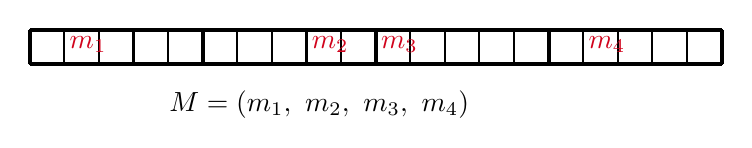
\begin{tikzpicture}[x=0.5pt,y=0.5pt,yscale=-1,xscale=1]
%uncomment if require: \path (0,88); %set diagram left start at 0, and has height of 88

%Shape: Grid [id:dp7159974501706334] 
\draw  [draw opacity=0][line width=0.75]  (15,13) -- (515,13) -- (515,38) -- (15,38) -- cycle ; \draw  [line width=0.75]  (40,13) -- (40,38)(65,13) -- (65,38)(90,13) -- (90,38)(115,13) -- (115,38)(140,13) -- (140,38)(165,13) -- (165,38)(190,13) -- (190,38)(215,13) -- (215,38)(240,13) -- (240,38)(265,13) -- (265,38)(290,13) -- (290,38)(315,13) -- (315,38)(340,13) -- (340,38)(365,13) -- (365,38)(390,13) -- (390,38)(415,13) -- (415,38)(440,13) -- (440,38)(465,13) -- (465,38)(490,13) -- (490,38) ; \draw  [line width=0.75]   ; \draw  [line width=0.75]  (15,13) -- (515,13) -- (515,38) -- (15,38) -- cycle ;
%Straight Lines [id:da4276676225384277] 
\draw [line width=1.5]    (15,38) -- (515,38) ;
%Straight Lines [id:da38414129135222486] 
\draw [line width=1.5]    (15,13) -- (515,13) ;
%Straight Lines [id:da8193193450080452] 
\draw [line width=1.5]    (15,38) -- (15,13) ;
%Straight Lines [id:da4559031610077283] 
\draw [line width=1.5]    (140,38) -- (140,13) ;
%Straight Lines [id:da7340056619830325] 
\draw [line width=1.5]    (515,38) -- (515,13) ;
%Straight Lines [id:da6116177459817139] 
\draw [line width=1.5]    (265,38) -- (265,13) ;
%Straight Lines [id:da4924257748666654] 
\draw [line width=1.5]    (390,38) -- (390,13) ;

% Text Node
\draw (42,16) node [anchor=north west][inner sep=0.75pt]   [align=left] {$\displaystyle \textcolor[rgb]{0.82,0.01,0.11}{m_{1}}$};
% Text Node
\draw (217,16) node [anchor=north west][inner sep=0.75pt]   [align=left] {$\displaystyle \textcolor[rgb]{0.82,0.01,0.11}{m}\textcolor[rgb]{0.82,0.01,0.11}{_{2}}$};
% Text Node
\draw (267,16) node [anchor=north west][inner sep=0.75pt]   [align=left] {$\displaystyle \textcolor[rgb]{0.82,0.01,0.11}{m}\textcolor[rgb]{0.82,0.01,0.11}{_{3}}$};
% Text Node
\draw (417,16) node [anchor=north west][inner sep=0.75pt]   [align=left] {$\displaystyle \textcolor[rgb]{0.82,0.01,0.11}{m}\textcolor[rgb]{0.82,0.01,0.11}{_{4}}$};
% Text Node
\draw (114,55) node [anchor=north west][inner sep=0.75pt]   [align=left] {$\displaystyle M=( m_{1} ,\ m_{2} ,\ m_{3} ,\ m_{4})$};


\end{tikzpicture}
}
\caption{Finding pivot $x$ using median of medians. The median of each subarray~(of size 5) is marked with $m_i$.
We then collect these medians and denote it as $M$. The median of $M$ will be the pivot $x$.}
\label{fig:median}
\end{figure}

There are two questions here. First, how to calculate the median of each subarray?
As each subarray is of size 5, we can use any algorithm. For example, we can sort it, using time of $5 \cdot \log 5$, to get its median.
Note, as there are $n/5$ subarrays, the total running time will be $n/5\cdot 5\cdot \log 5 = \log 5\cdot n = \Theta(n)$.
Second, how to calcuate the median of $M$? The answer is a recursive call: selection~($M$, $|M|/2$).
We will see later on that, the resulting algorithm still runs in linear time.

The pseudo-code for find-pivot function is given below.

\begin{minipage}{0.8\textwidth}
	\aaA {6}{function find-pivot~($A$)}\xxx
	\aab {\textcolor{blue}{if $|A| < 5$: find~(e.g., by sorting $A$) and return the median of $A$;}}\xxx
	\aab {partition $A$ into $n/5$ subarrays of size 5;}\xxx
	\aab {calculate the median of each subarray;}\xxx
	\aab {let $M$ be the array that includes all medians;}\xxx
	\aab {return selection~($M$, $|M|/2$);}\xxx
	\aaa {end algorithm;}\xxx
\end{minipage}

